%!TEX TS-program = lualatex
%!TEX encoding   = UTF-8 Unicode

\documentclass[aspectratio=169]{beamer}

\usefonttheme{default}
\usefonttheme{professionalfonts}

\usepackage{booktabs}
\usepackage{dsfont}
\usepackage{fontspec}
\usepackage{multirow}
\usepackage{mathpazo}
\usepackage{manfnt}
\usepackage{pifont}
\usepackage{siunitx}
\usepackage{tabularx}
\usepackage{xspace}

% Define new column type in tabularx environment, that combines the X-cell with the c-cell
\newcolumntype{Y}{>{\centering\arraybackslash}X}

\usepackage{appendixnumberbeamer}

\usepackage[T1]{fontenc}

\sisetup{
  detect-weight           = true,
  detect-inline-weight    = math,
  separate-uncertainty    = true,
  table-align-uncertainty = true,
  table-text-alignment    = center,
}

\defaultfontfeatures{
    Ligatures = TeX, % Ensures that dashes etc. are typeset properly
    %Numbers   = {%
    %  Monospaced,    % Always use monospaced numbers
    %  Lining         % Always use lining numbers
    %},
}

\usepackage[british]{babel}

%%%%%%%%%%%%%%%%%%%%%%%%%%%%%%%%%%%%%%%%%%%%%%%%%%%%%%%%%%%%%%%%%%%%%%%%
% Mathematics
%%%%%%%%%%%%%%%%%%%%%%%%%%%%%%%%%%%%%%%%%%%%%%%%%%%%%%%%%%%%%%%%%%%%%%%%

\usepackage{amsmath}
\usepackage{amssymb}

% Use bold font to indicate vectors
\let\vec\mathbf

\newcommand{\betti}        [1]{\ensuremath{\beta_{#1}}}
\newcommand{\diagram}         {\ensuremath{\mathcal{D}}}
\newcommand{\featurevector}[1]{\ensuremath{\mathcal{F}_{#1}}}
\newcommand{\graph}           {\ensuremath{\mathcal{G}}}
\newcommand{\landau}       [1]{\ensuremath{\mathcal{O}\left(#1\right)}}
\newcommand{\real}            {\ensuremath{\mathds{R}}}

\DeclareMathOperator{\ccount}     {\mathfrak{z}} % persistent cycle counter function
\DeclareMathOperator{\dist}       {dist}         % distance functor
\DeclareMathOperator{\flabel}     {l}            % label function
\DeclareMathOperator{\pcount}     {\mathfrak{p}} % persistent counter function
\DeclareMathOperator{\persistence}{pers}         % persistence function

\let\originalleft\left
\let\originalright\right
\renewcommand{\left}{\mathopen{}\mathclose\bgroup\originalleft}
\renewcommand{\right}{\aftergroup\egroup\originalright}

%%%%%%%%%%%%%%%%%%%%%%%%%%%%%%%%%%%%%%%%%%%%%%%%%%%%%%%%%%%%%%%%%%%%%%%%
% Plots & graphics
%%%%%%%%%%%%%%%%%%%%%%%%%%%%%%%%%%%%%%%%%%%%%%%%%%%%%%%%%%%%%%%%%%%%%%%%

\usepackage[absolute,overlay]{textpos}

\usepackage{tikz}
\usepackage{pgfplots}

\usepgfplotslibrary{external}
\usepgfplotslibrary{groupplots}

\tikzexternalize
\tikzsetexternalprefix{Figures/External/}

\pgfplotsset{compat=1.16}

\definecolor{cardinal} {RGB}{196, 30, 58}
\definecolor{lightgrey}{RGB}{230,230,230}

\pgfplotsset{%
  /pgfplots/colormap={mlcb}{rgb255=(196,30,58) rgb255=(80,200,120) rgb255=(49,140,231)}
}

%%%%%%%%%%%%%%%%%%%%%%%%%%%%%%%%%%%%%%%%%%%%%%%%%%%%%%%%%%%%%%%%%%%%%%%%
% Theming
%%%%%%%%%%%%%%%%%%%%%%%%%%%%%%%%%%%%%%%%%%%%%%%%%%%%%%%%%%%%%%%%%%%%%%%%

\setsansfont{Myriad Pro}
\setmonofont{Hack}

\setbeamercolor{alerted text}           {fg=cardinal      }
\setbeamercolor{bibliography entry note}{fg=black         }
\setbeamercolor{structure}              {fg=black,bg=white}
\setbeamercolor{normal text}            {fg=black,bg=white}
\setbeamercolor{frametitle}             {fg=black,bg=white}
\setbeamercolor{item projected}         {fg=white,bg=black}
\setbeamercolor{footline colour}        {fg=black,bg=white}

\setbeamertemplate{caption}                         {\insertcaption}
\setbeamertemplate{itemize items}[circle]

% Workaround for text bullets that are too large. I do not know their
% root cause.
\setbeamertemplate{itemize items}{%
  \textbullet
}

\setbeamertemplate{enumerate items}   [square]
\setbeamertemplate{navigation symbols}              {}

%\setbeamerfont{title}     {family=\fontspec{Libre Franklin Bold}}
%\setbeamerfont{frametitle}{family=\fontspec{Libre Franklin Bold}}
%\setbeamerfont{author}    {family=\fontspec{Libre Franklin Bold}}

\setbeamertemplate{footline}{%
  \leavevmode%
  \hbox{%
    \begin{beamercolorbox}[wd=.075\paperwidth, ht=2.5ex, dp=2ex, left]{footline colour}%
      \hspace*{2.5mm}
\includegraphics[height=1.5ex]{Figures/Logo_D-BSSE}%
    \end{beamercolorbox}%
    \begin{beamercolorbox}[wd=.925\paperwidth, ht=2.5ex, dp=2ex, right]{footline colour}%
      \usebeamerfont{title in head/foot}\insertshorttitle%
      \hspace*{3.14mm}%
      \hspace*{3.14mm}\insertdate%
      \hspace*{4.5mm}%
    \end{beamercolorbox}%
  }
}

% Disable rules for footnotes; this makes the display less cluttered in my opinion.
\renewcommand{\footnoterule}{}

\makeatletter
\addtobeamertemplate{block begin}{
\def\@listi{\leftmargin\leftmargini
              \topsep    0pt
              \parsep    0pt
              \itemsep   3pt plus 2pt minus 3pt}
\partopsep 0pt
}
\makeatother

\AtBeginSection[]
{
  \begin{frame}<beamer>
    \vfill
    \begin{center}
      \usebeamerfont{title}%
      \begin{huge}
        \insertsectionhead%
      \end{huge}
    \end{center}
    \vfill
  \end{frame}
}

%%%%%%%%%%%%%%%%%%%%%%%%%%%%%%%%%%%%%%%%%%%%%%%%%%%%%%%%%%%%%%%%%%%%%%%%
% Algorithms
%%%%%%%%%%%%%%%%%%%%%%%%%%%%%%%%%%%%%%%%%%%%%%%%%%%%%%%%%%%%%%%%%%%%%%%%

\usepackage{algorithm}
\usepackage{algorithmicx}
\usepackage{algpseudocode}

%%%%%%%%%%%%%%%%%%%%%%%%%%%%%%%%%%%%%%%%%%%%%%%%%%%%%%%%%%%%%%%%%%%%%%%%
% Typography
%%%%%%%%%%%%%%%%%%%%%%%%%%%%%%%%%%%%%%%%%%%%%%%%%%%%%%%%%%%%%%%%%%%%%%%%

\renewcommand{\th}{\textsuperscript{\textup{th}}\xspace}

\newcommand{\yes}{\textcolor{eth-4}{\ding{51}}}
\newcommand{\no} {\textcolor{eth-7}{\ding{55}}}

\def\signed #1{{\leavevmode\unskip\nobreak\hfil\penalty50\hskip1em
  \hbox{}\nobreak\hfill #1%
  \parfillskip=0pt \finalhyphendemerits=0 \endgraf}}

\newsavebox\mybox
\newenvironment{aquote}[1]
  {\savebox\mybox{\scriptsize#1}``\hspace*{-.25ex}}
  {\unskip''\vspace*{1mm}\signed{\usebox\mybox}}

%%%%%%%%%%%%%%%%%%%%%%%%%%%%%%%%%%%%%%%%%%%%%%%%%%%%%%%%%%%%%%%%%%%%%%%%
% Title
%%%%%%%%%%%%%%%%%%%%%%%%%%%%%%%%%%%%%%%%%%%%%%%%%%%%%%%%%%%%%%%%%%%%%%%%

\title{Machine Learning for Biology}
\subtitle{Workshop, D-BSSE Retreat}
\author{%
  Anja Gumpinger \and Catherine Jutzeler \and Bastian Rieck \and Caroline Weis
}
\date{28 June 2019}

%%%%%%%%%%%%%%%%%%%%%%%%%%%%%%%%%%%%%%%%%%%%%%%%%%%%%%%%%%%%%%%%%%%%%%%%
% Slides
%%%%%%%%%%%%%%%%%%%%%%%%%%%%%%%%%%%%%%%%%%%%%%%%%%%%%%%%%%%%%%%%%%%%%%%%

\begin{document}

  \begin{frame}[plain]
    \maketitle
  \end{frame}

  \section{What is machine learning?}

  \begin{frame}{Group work 1}
    \begin{itemize}
        \item What is machine learning?
        \item Which machine learning techniques do you already know?
    \end{itemize}
    %
    \vfill
    %
    \textbf{Instructions}: please discuss the questions above within
    your group. Use the provided pens and sheets to write down your
    answers.~($\approx\SI{5}{\minute}$)
  \end{frame}

  \begin{frame}{Machine learning~(ML)}
    \begin{aquote}{Arthur Samuel, Computer Scientist, 1959}
      Machine learning is the field of study that gives the computer the
      \emph{ability to learn without being explicitly programmed}.
    \end{aquote}
    %
    \pause
    \vfill
    %
    \begin{aquote}{Tom Mitchell, Computer Scientist, 1997}
      A computer program is said to \emph{learn from Experience E} with respect
      to some \emph{class of Task T} and some \emph{performance measure
      P}, if its performance on T, as measured by P, improves with \emph{Experience
      E}.
    \end{aquote}
  \end{frame}

  \begin{frame}{Everyday applications of machine learning}
    \begin{columns}
      \column{0.25\linewidth}
        \onslide<1->{%
          \begin{figure}
            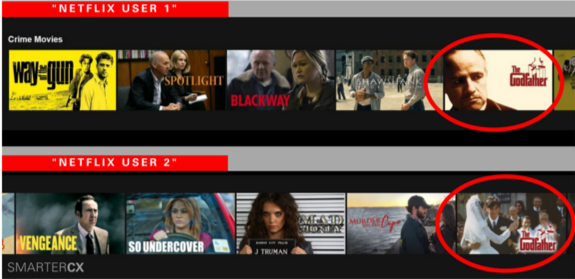
\includegraphics[width=\linewidth]{Figures/Netflix}
            \caption{\scriptsize Personalised entertainment recommendations}
          \end{figure}
        }
      \column{0.25\linewidth}
        \onslide<2->{%
          \begin{figure}
            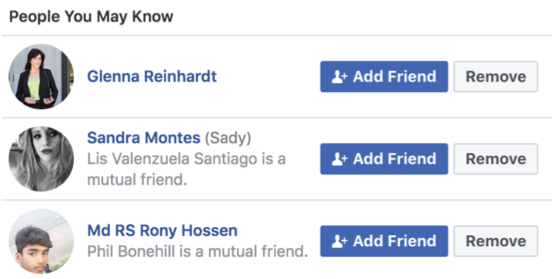
\includegraphics[width=\linewidth]{Figures/Facebook}
            \caption{\scriptsize Personalised contact recommendations}
          \end{figure}
        }
      \column{0.25\linewidth}
        \onslide<3->{%
          \begin{figure}
            
\includegraphics[width=\linewidth]{Figures/Shazaam}
            \caption{\scriptsize Music recognition}
          \end{figure}
        }
      \column{0.25\linewidth}
        \onslide<4->{%
          \begin{figure}
            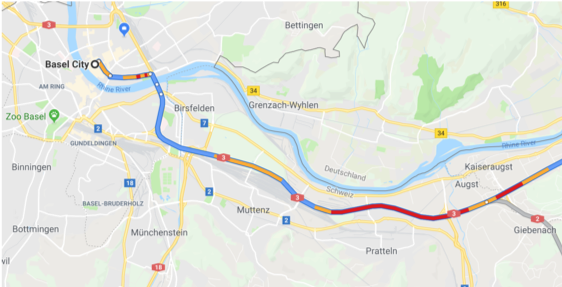
\includegraphics[width=\linewidth]{Figures/Google}
            \caption{\scriptsize Traffic prediction}
          \end{figure}
        }
    \end{columns}
  \end{frame}

  \begin{frame}{Biological applications of machine learning}
    \begin{itemize}
      \item Identifying gene coding regions
      \item Protein structure prediction~(proteomics)
      \item Function prediction based on sequences
      \item Gene classification
      \item Motif detection
    \end{itemize}
  \end{frame}

  \begin{frame}{A bestiary for machine learning}
    \begin{figure}
      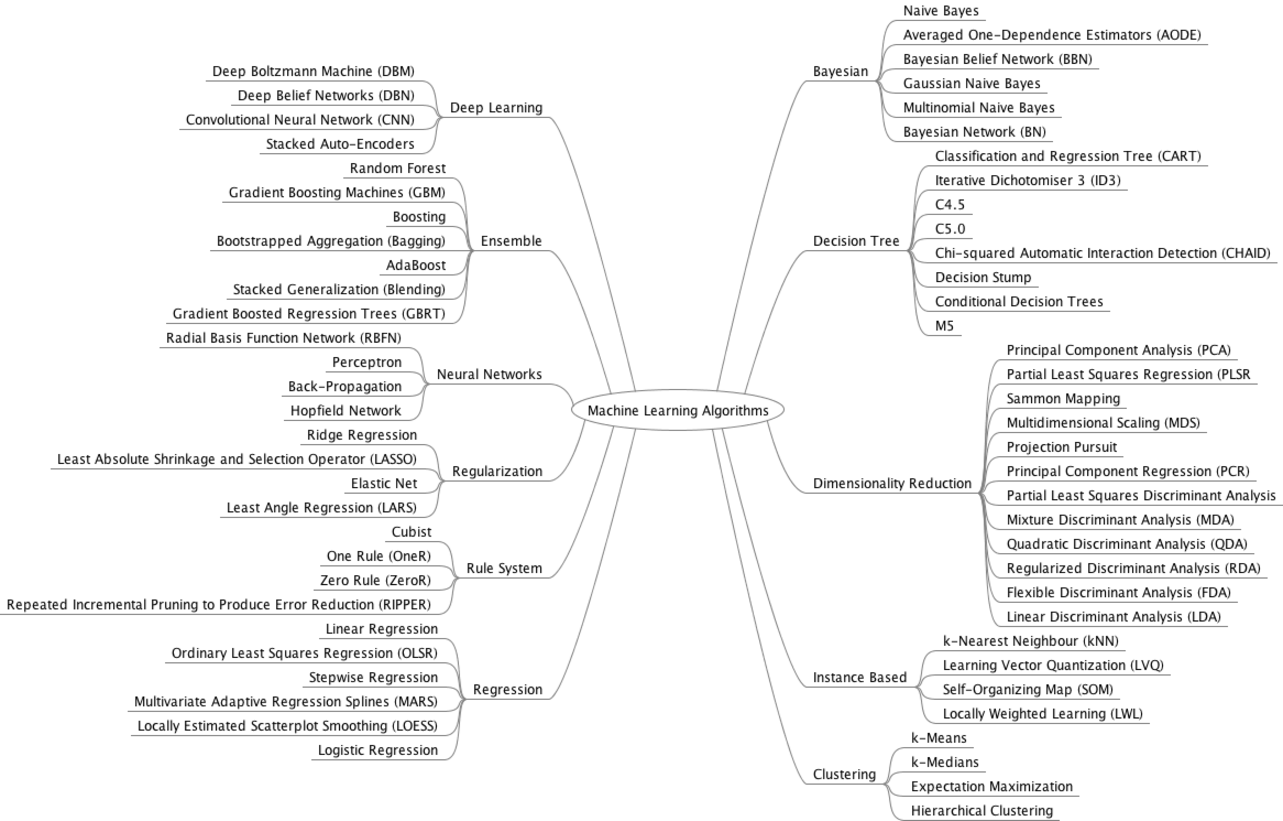
\includegraphics[width=0.75\linewidth]{Figures/Zoo}
    \end{figure}
  \end{frame}

  \begin{frame}{}
    \begin{figure}
      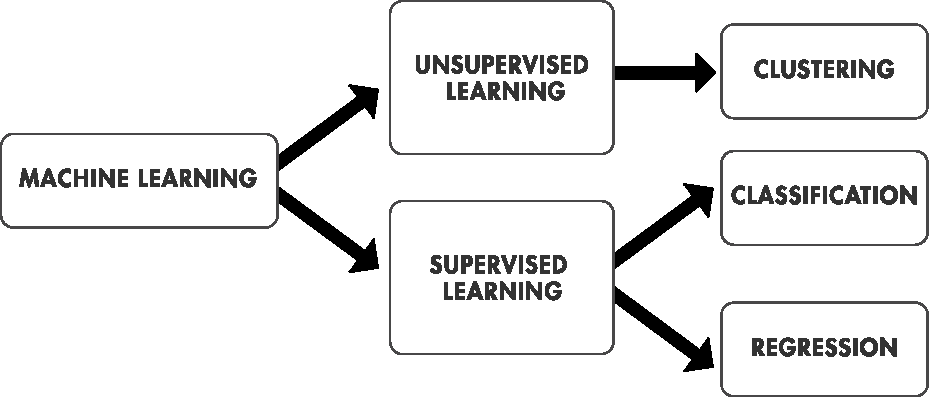
\includegraphics[width=0.75\linewidth]{Figures/Machine_learning_pipeline}
    \end{figure}
  \end{frame}

  \section{Clustering methods}

  \begin{frame}{Machine leaning and candy}{A good fit}
    \begin{figure}
      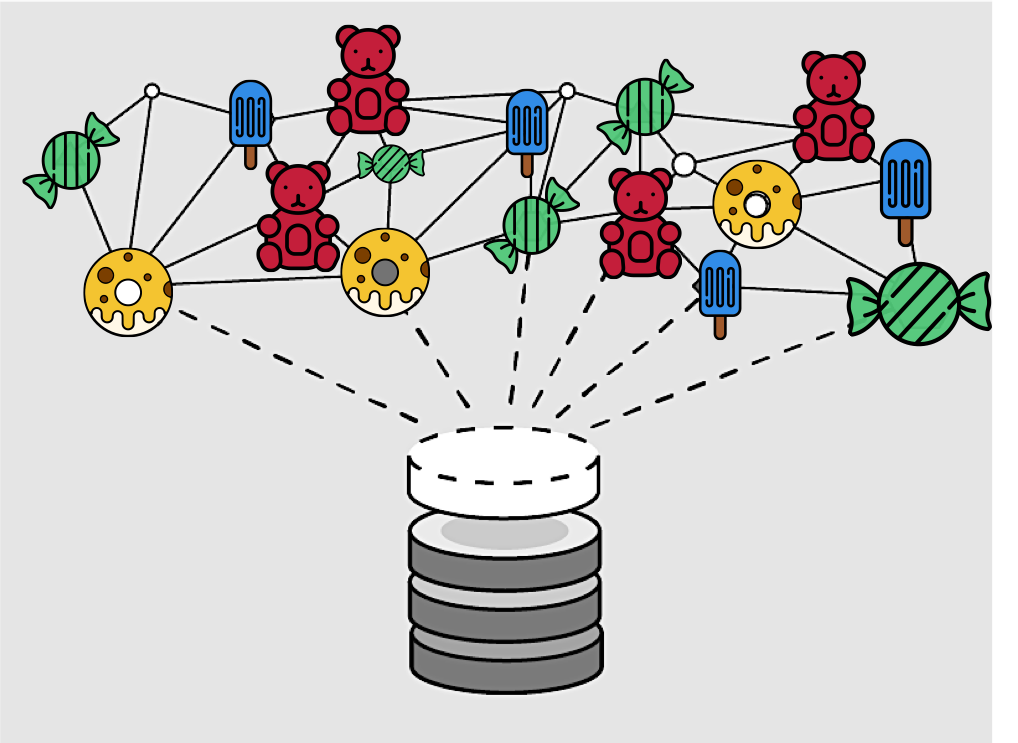
\includegraphics[width=0.50\linewidth]{Figures/Introduction}
    \end{figure}
  \end{frame}
  
  \begin{frame}{What is clustering?}

    \begin{block}{Problem definition}
      Given a set of $n$ objects, how can we group them into $k$
      clusters, such that all objects in one cluster are more
      \emph{similar} to each other than to the objects in the
      remaining clusters?
    \end{block}

    \vfill

    \begin{itemize}
      \item \emph{Unsupervised} technique: labels are not known
      \item Some parameter choices:
        \begin{itemize}
          \item How many clusters?
          \item How to measure similarity?
        \end{itemize}
    \end{itemize}
  \end{frame}

  \begin{frame}{Group work 2}{Candy mountain clustering}
    \begin{figure}
      \includegraphics[width=0.50\linewidth]{Figures/Candy_mountain}
    \end{figure}
  \end{frame}

  \begin{frame}{Some constraints}
    \begin{columns}
      \column{0.30\linewidth}
        \begin{figure}
          \includegraphics[width=\linewidth]{Figures/Candy_mountain}
        \end{figure}
      \column{0.70\linewidth}
        \begin{itemize}
          \item There are $n = 48$ objects
          \item Let us assume we want $k = 4$ clusters
          \item There are $S(48, 4) = 3301160143687238289723531701$ ways
            of doing so:
            %
            \begin{scriptsize}
              three octillion, three hundred one septillion, one hundred
              sixty sextillion, one hundred forty three quintillion, six
              hundred eighty seven quadrillion, two hundred thirty eight
              trillion, two hundred eighty nine billion, seven hundred
              twenty three million, five hundred thirty one thousand,
              seven hundred one
            \end{scriptsize}
        \end{itemize}
    \end{columns}
  \end{frame}

  \begin{frame}{}
    \begin{center}
      \begin{huge}
        There is no \emph{best} clustering.
      \end{huge}
    \end{center}
  \end{frame}

  \begin{frame}{?}
    \begin{figure}
      \includegraphics[width=0.75\linewidth]{Figures/Clustering_by_colour}
    \end{figure}
  \end{frame}

  \begin{frame}{Clustering by colour~($k = 4$)}
    \begin{figure}
      \includegraphics[width=0.75\linewidth]{Figures/Clustering_by_colour}
    \end{figure}
  \end{frame}

  \begin{frame}{?}
    \begin{figure}
      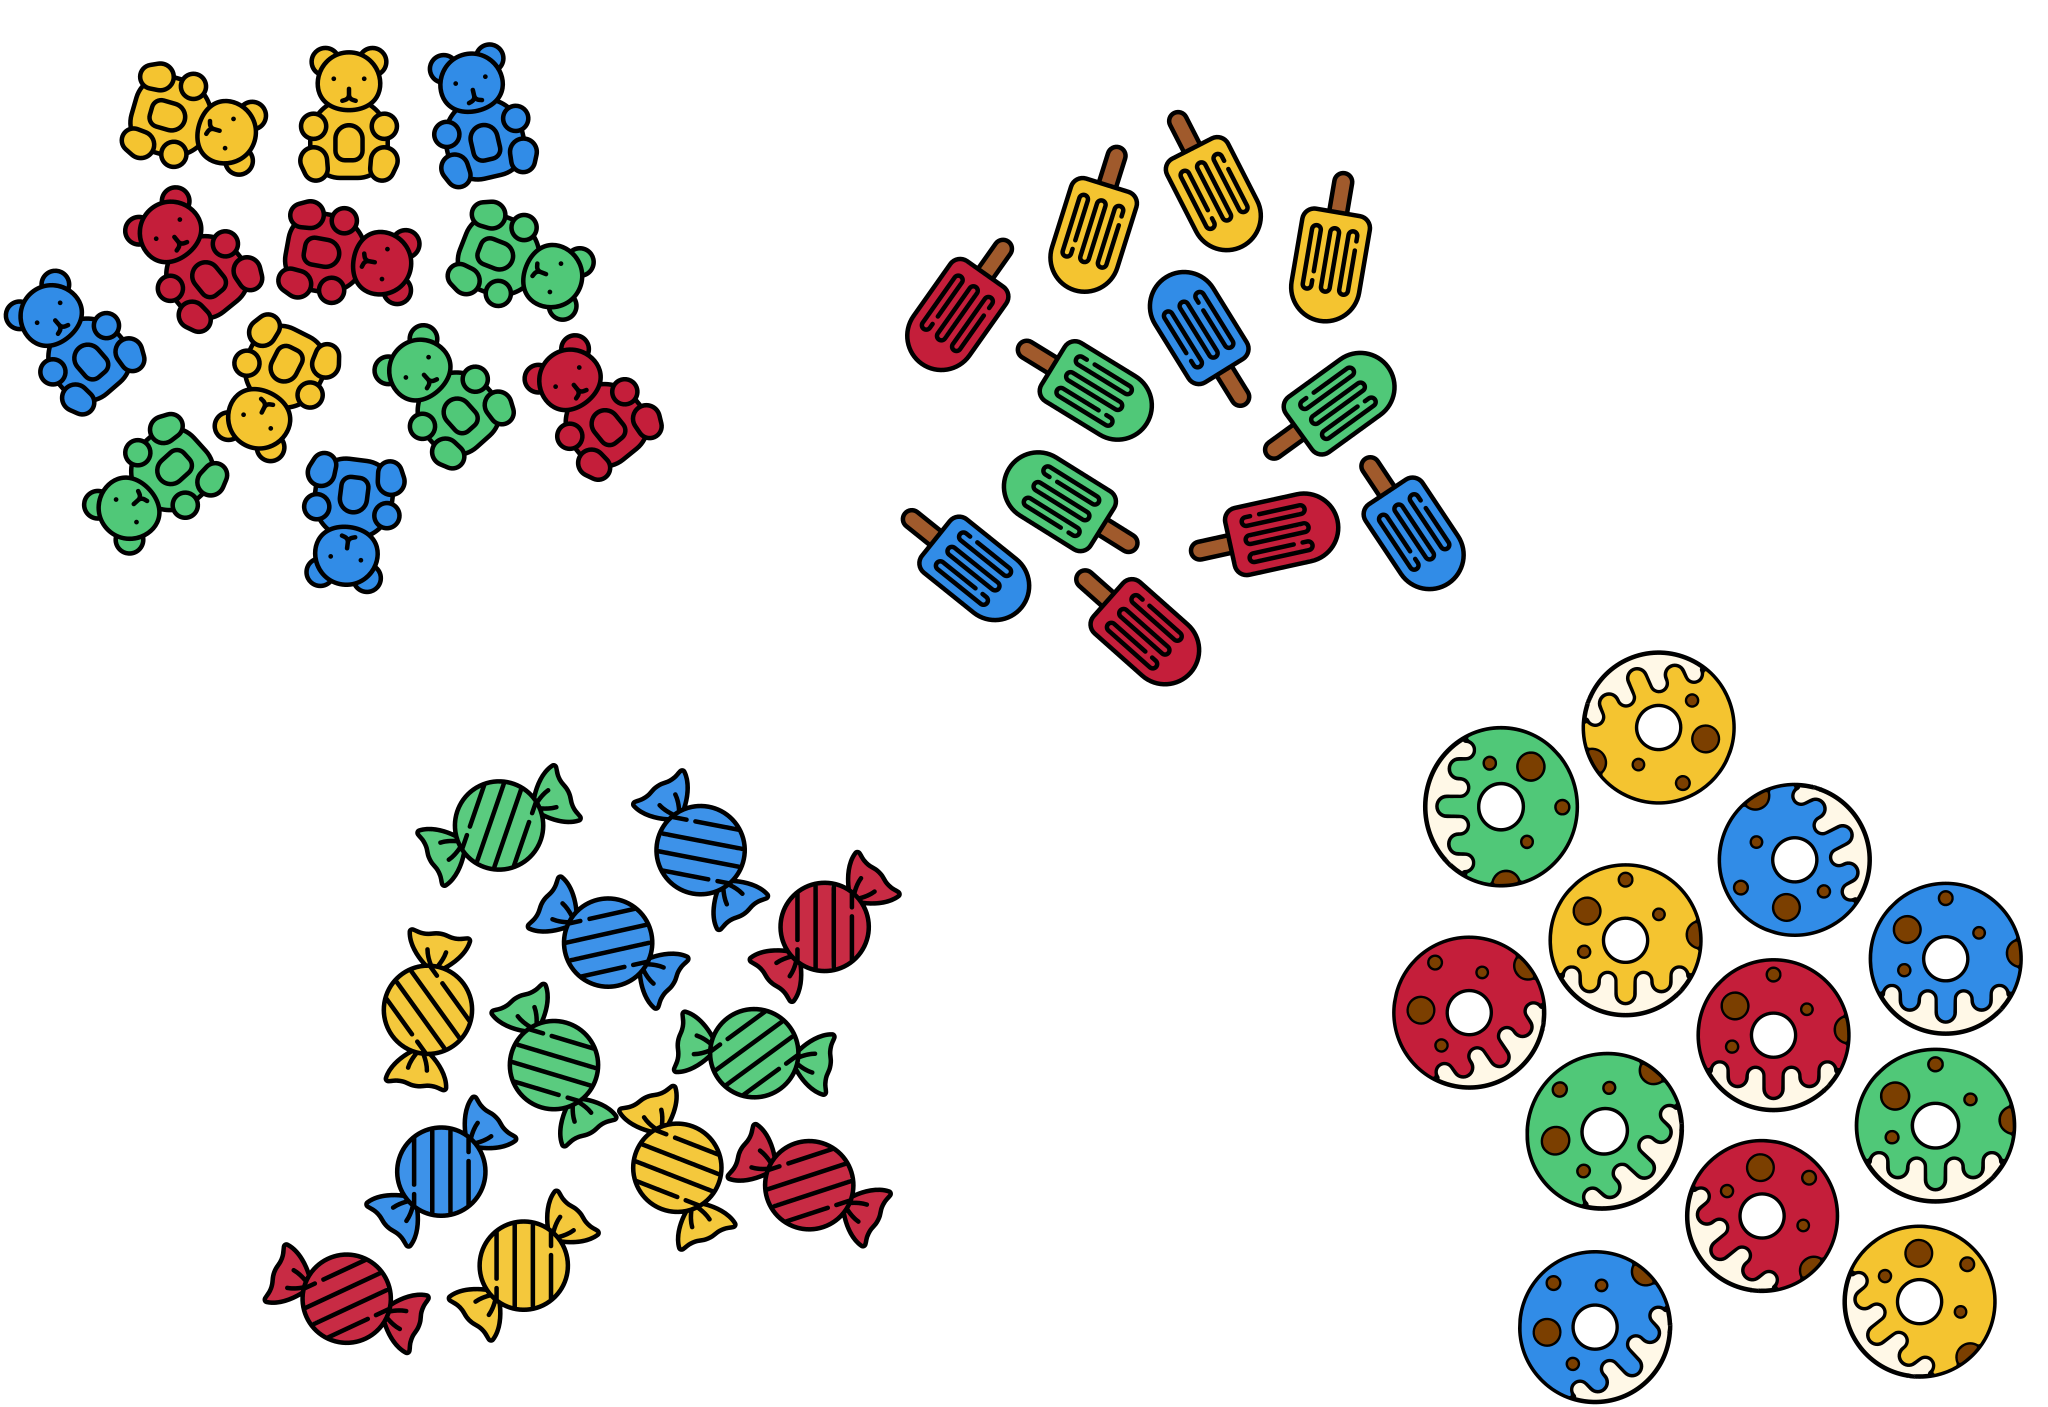
\includegraphics[width=0.75\linewidth]{Figures/Clustering_by_type}
    \end{figure}
  \end{frame}

  \begin{frame}{Clustering by type~($k = 4)$}
    \begin{figure}
      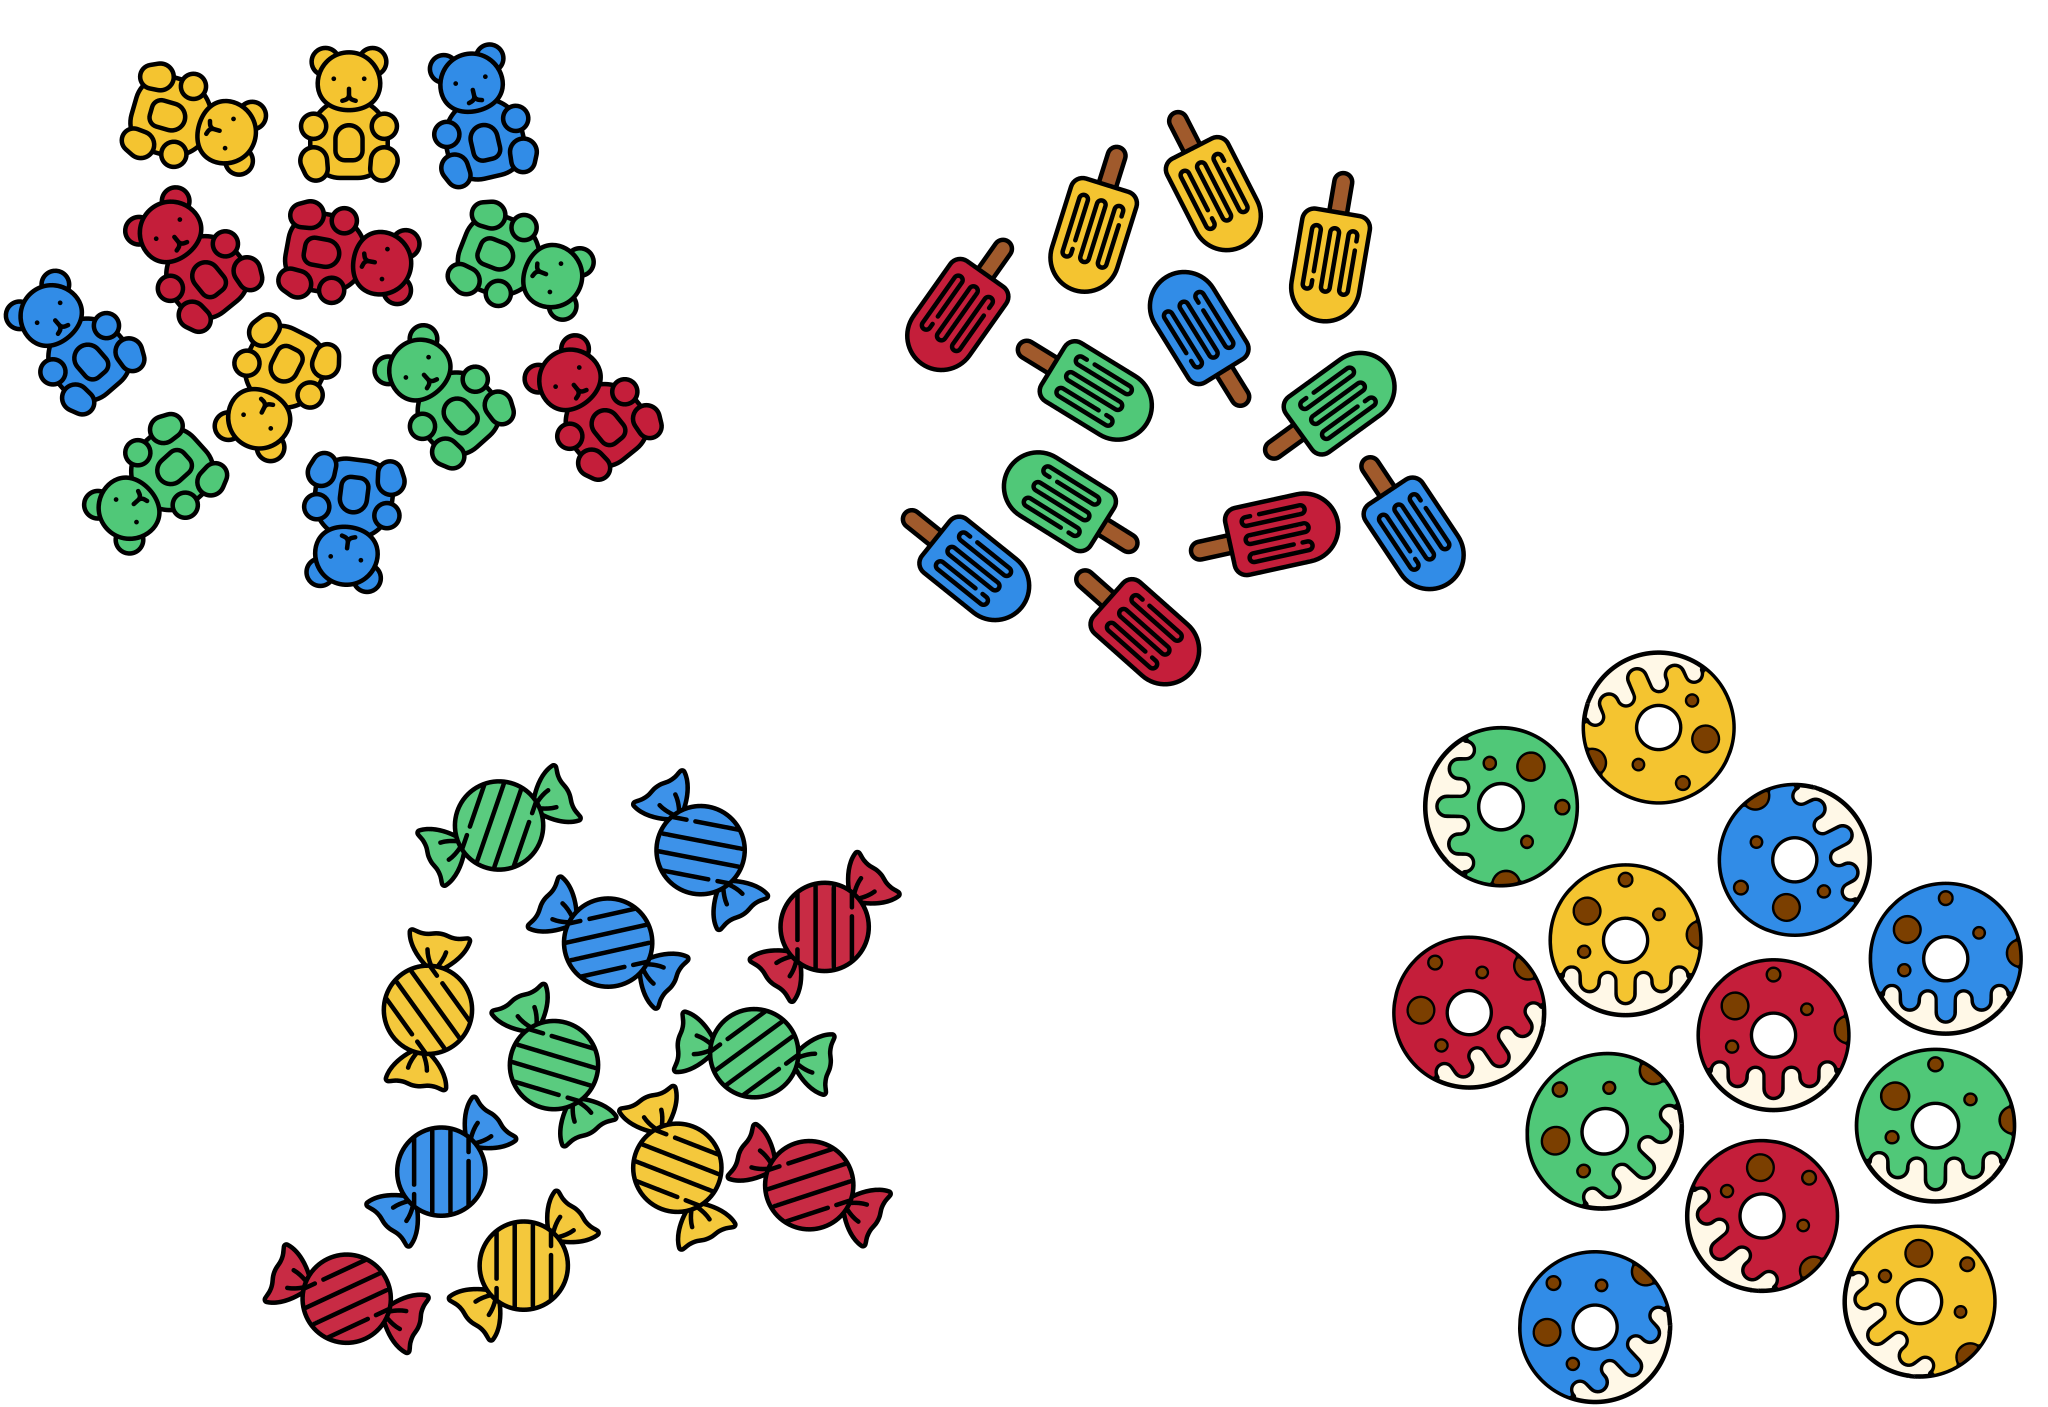
\includegraphics[width=0.75\linewidth]{Figures/Clustering_by_type}
    \end{figure}
  \end{frame}

  \begin{frame}{?}
    \begin{figure}
      \includegraphics[width=0.75\linewidth]{Figures/Clustering_by_topology}
    \end{figure}
  \end{frame}

  \begin{frame}{Clustering by topology~($k = 2)$}
    \begin{figure}
      \includegraphics[width=0.75\linewidth]{Figures/Clustering_by_topology}
    \end{figure}
  \end{frame}

  \begin{frame}{?}
    \begin{figure}
      \includegraphics[width=0.75\linewidth]{Figures/Clustering_by_ingredients}
    \end{figure}
  \end{frame}

  \begin{frame}{Clustering by ingredients~($k = 2)$}
    \begin{figure}
      \includegraphics[width=0.75\linewidth]{Figures/Clustering_by_ingredients}
    \end{figure}
  \end{frame}

  \begin{frame}{A selection of clustering methods}
    \begin{itemize}
      \item Hierarchical clustering~(agglomerative, divisive, \dots)
      \item \texttt{$k$-means}
      \item Density-based clustering~(\texttt{DBSCAN}, \texttt{DENCLUE})
    \end{itemize}
  \end{frame}


  \begin{frame}
    \begin{figure}
      \begin{tikzpicture}
        \tikzset{%
          every mark/.append style = {
            mark size = 0.35pt,
          }
        }
        %
        \pgfplotsset{%
          /pgfplots/scatter/use mapped color = {
            draw = mapped color,
            fill = mapped color,
          }
        }
        %
        \begin{groupplot}[%
          group style = {%
            group size     = 3 by 4,
            horizontal sep = 0pt,
            vertical sep   = 0pt,
          },
          %
          axis lines = none,
          clip mode  = individual,
          height     = 3.5cm,
          width      = 3.5cm,
        ]
          \nextgroupplot
            \addplot[%
              scatter,
              only marks,
              point meta=explicit
            ] table[meta index=2] {Data/AgglomerativeClustering_0.txt};
            \node at (rel axis cs:0.5,1.075) {\small Agglomerative};

          \nextgroupplot

            \addplot[%
              scatter,
              only marks,
              point meta=explicit
            ] table[meta index=2] {Data/MiniBatchKMeans_0.txt};
            \node at (rel axis cs:0.5,1.10) {\small\texttt{$k$-means}};

          \nextgroupplot

            \addplot[%
              scatter,
              only marks,
              point meta=explicit
            ] table[meta index=2] {Data/DBSCAN_0.txt};
            \node at (rel axis cs:0.5,1.10) {\small\texttt{DBSCAN}};

          \nextgroupplot
            \addplot[%
              scatter,
              only marks,
              point meta=explicit
            ] table[meta index=2] {Data/AgglomerativeClustering_1.txt};

          \nextgroupplot

            \addplot[%
              scatter,
              only marks,
              point meta=explicit
            ] table[meta index=2] {Data/MiniBatchKMeans_1.txt};

          \nextgroupplot

            \addplot[%
              scatter,
              only marks,
              point meta=explicit
            ] table[meta index=2] {Data/DBSCAN_1.txt};

          \nextgroupplot
            \addplot[%
              scatter,
              only marks,
              point meta=explicit
            ] table[meta index=2] {Data/AgglomerativeClustering_2.txt};

          \nextgroupplot

            \addplot[%
              scatter,
              only marks,
              point meta=explicit
            ] table[meta index=2] {Data/MiniBatchKMeans_2.txt};

          \nextgroupplot

            \addplot[%
              scatter,
              only marks,
              point meta=explicit
            ] table[meta index=2] {Data/DBSCAN_2.txt};

          \nextgroupplot
            \addplot[%
              scatter,
              only marks,
              point meta=explicit
            ] table[meta index=2] {Data/AgglomerativeClustering_5.txt};

          \nextgroupplot

            \addplot[%
              scatter,
              only marks,
              point meta=explicit
            ] table[meta index=2] {Data/MiniBatchKMeans_5.txt};

          \nextgroupplot

            \addplot[%
              scatter,
              only marks,
              point meta=explicit
            ] table[meta index=2] {Data/DBSCAN_5.txt};

        \end{groupplot}
      \end{tikzpicture}
    \end{figure}
  \end{frame}

  \begin{frame}{Similarity measures}
    \begin{center}
      \begin{tabular}{ll}
        \toprule
        \emph{Which metric should I use for}\dots? & \\
        \midrule
        Continuous data~({\small temperature, length, \dots}) & Euclidean distance, Mahalanobis distance\\
        Categorical data~({\small blood type, sex, \dots})    & Hamming distance\\
        Images                                                & Euclidean distance~(?)\\
        Graphs                                                & Weisfeiler--Lehman graph kernels\\
        Time series                                           & Dynamic time warping~(DTW)\\
        \bottomrule
      \end{tabular}
    \end{center}
  \end{frame}

  \begin{frame}{How to choose $k$?}
    \begin{itemize}
      \item \emph{$\beta$-CV}: ratio of mean intracluster distance to mean intercluster distance
      \item \emph{C index}: ratio of intracluster distances to sum of the largest distances between points
      \item \emph{Dunn index}: ratio of smallest distance between points in different clusters to largest diameter of a cluster
      \item \emph{Silhouette score}: ensures that clusters are \emph{cohesive} while also being \emph{separate}
    \end{itemize}
    %
    \vfill
    %
    All of these measures have their shortcomings, though, and can be
    ``tricked''. Ideally, ground truth information is available to
    verify a clustering.
  \end{frame}

  \section{Classification methods}

\begin{frame}{Classification}
    \textbf{Problem}:
    \newline
    Identify a new object based on previously seen objects of similar type.
    \newline\newline
    \noindent
    \textbf{Properties}:
    \begin{itemize}
        \item instance of \textit{supervised} machine learning, i.e. requires \textit{labels} for data points
        \item requires \textit{training}, i.e. presentation of examples to an algorithm
        \item \textit{prediction}, i.e. the prediction of the label for previously unseen data points
    \end{itemize}
\end{frame}

\begin{frame}{Classification - Concept: Training}
    \begin{figure}
        \centering
        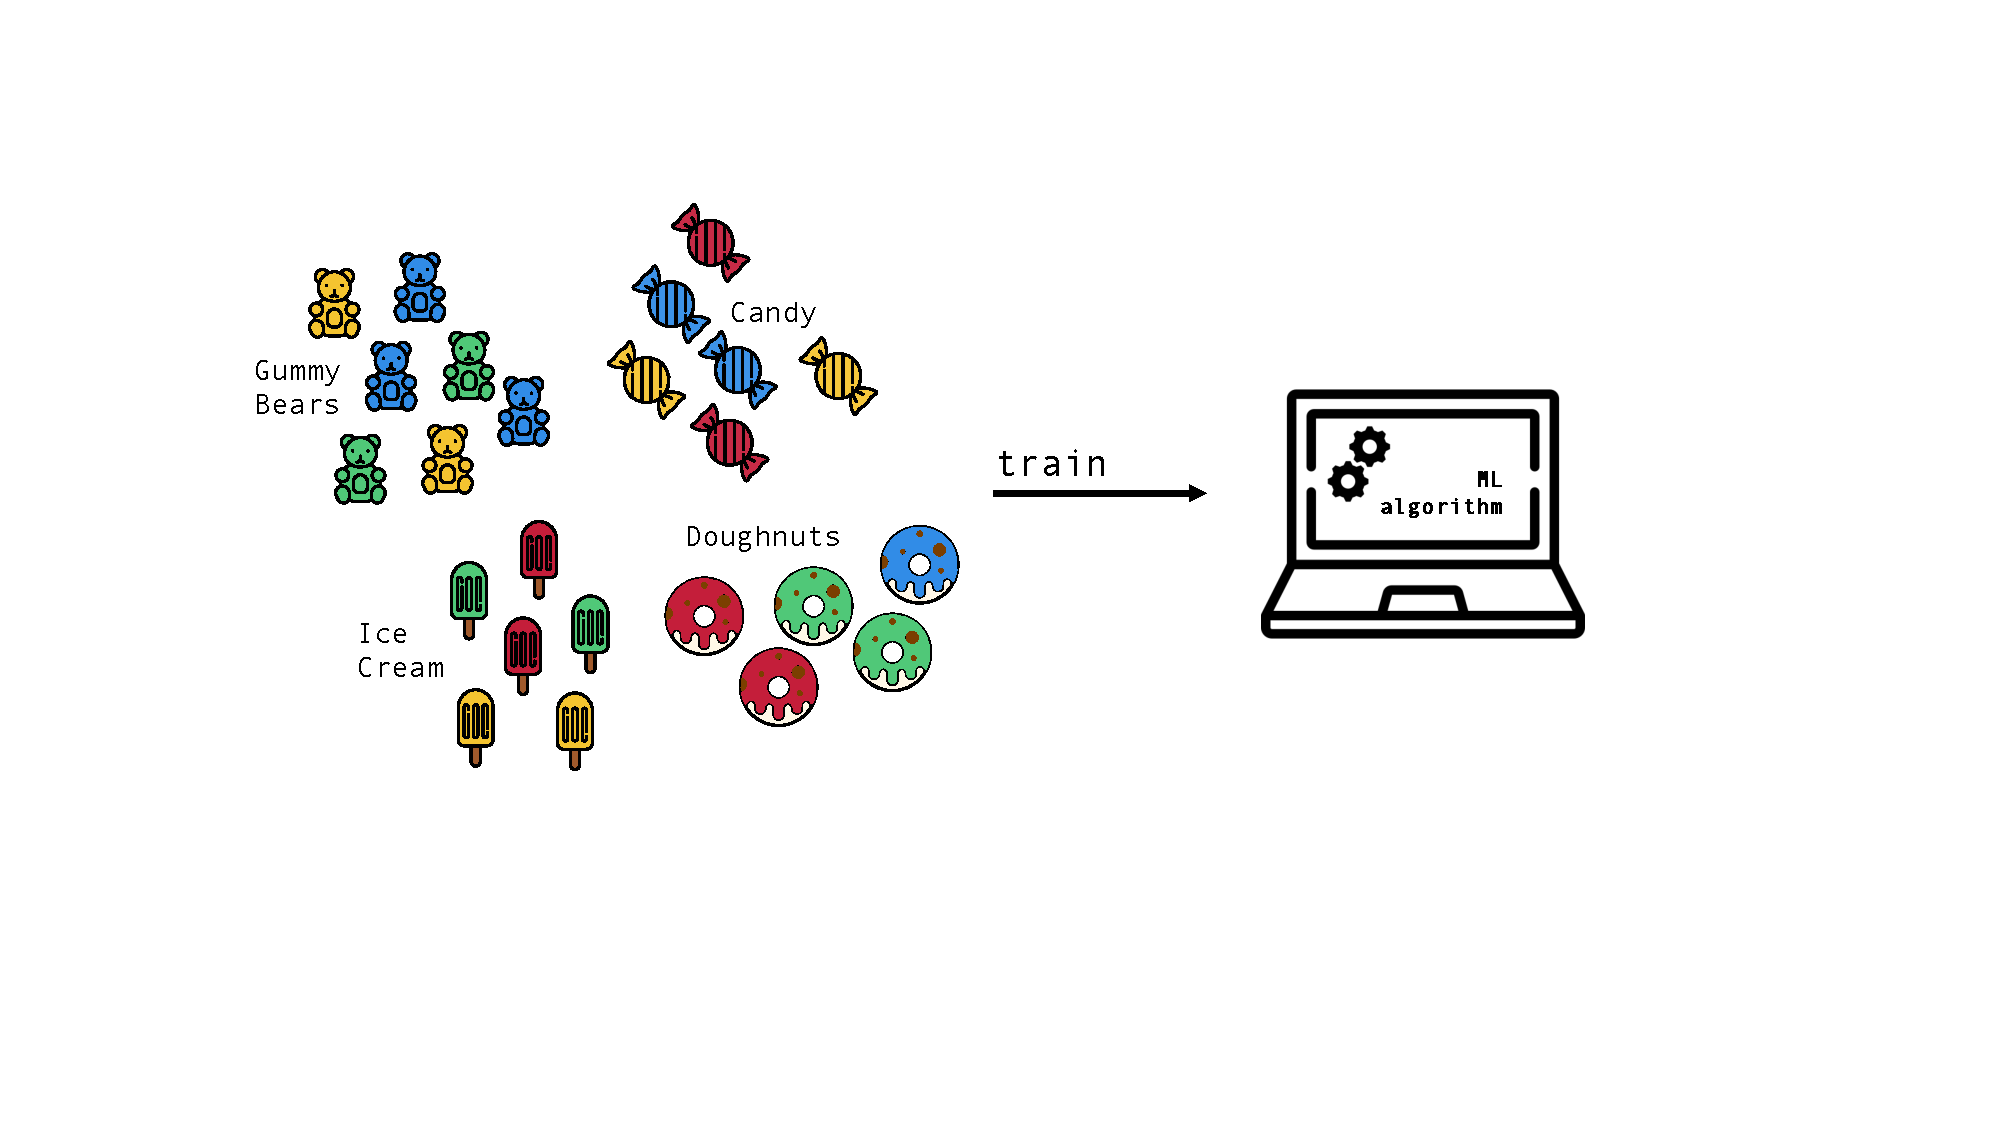
\includegraphics[scale=0.5]{Figures/example_training.pdf}
    \end{figure}
\end{frame}

\begin{frame}{Classification - Concept: Prediction}
    \begin{figure}
        \centering
        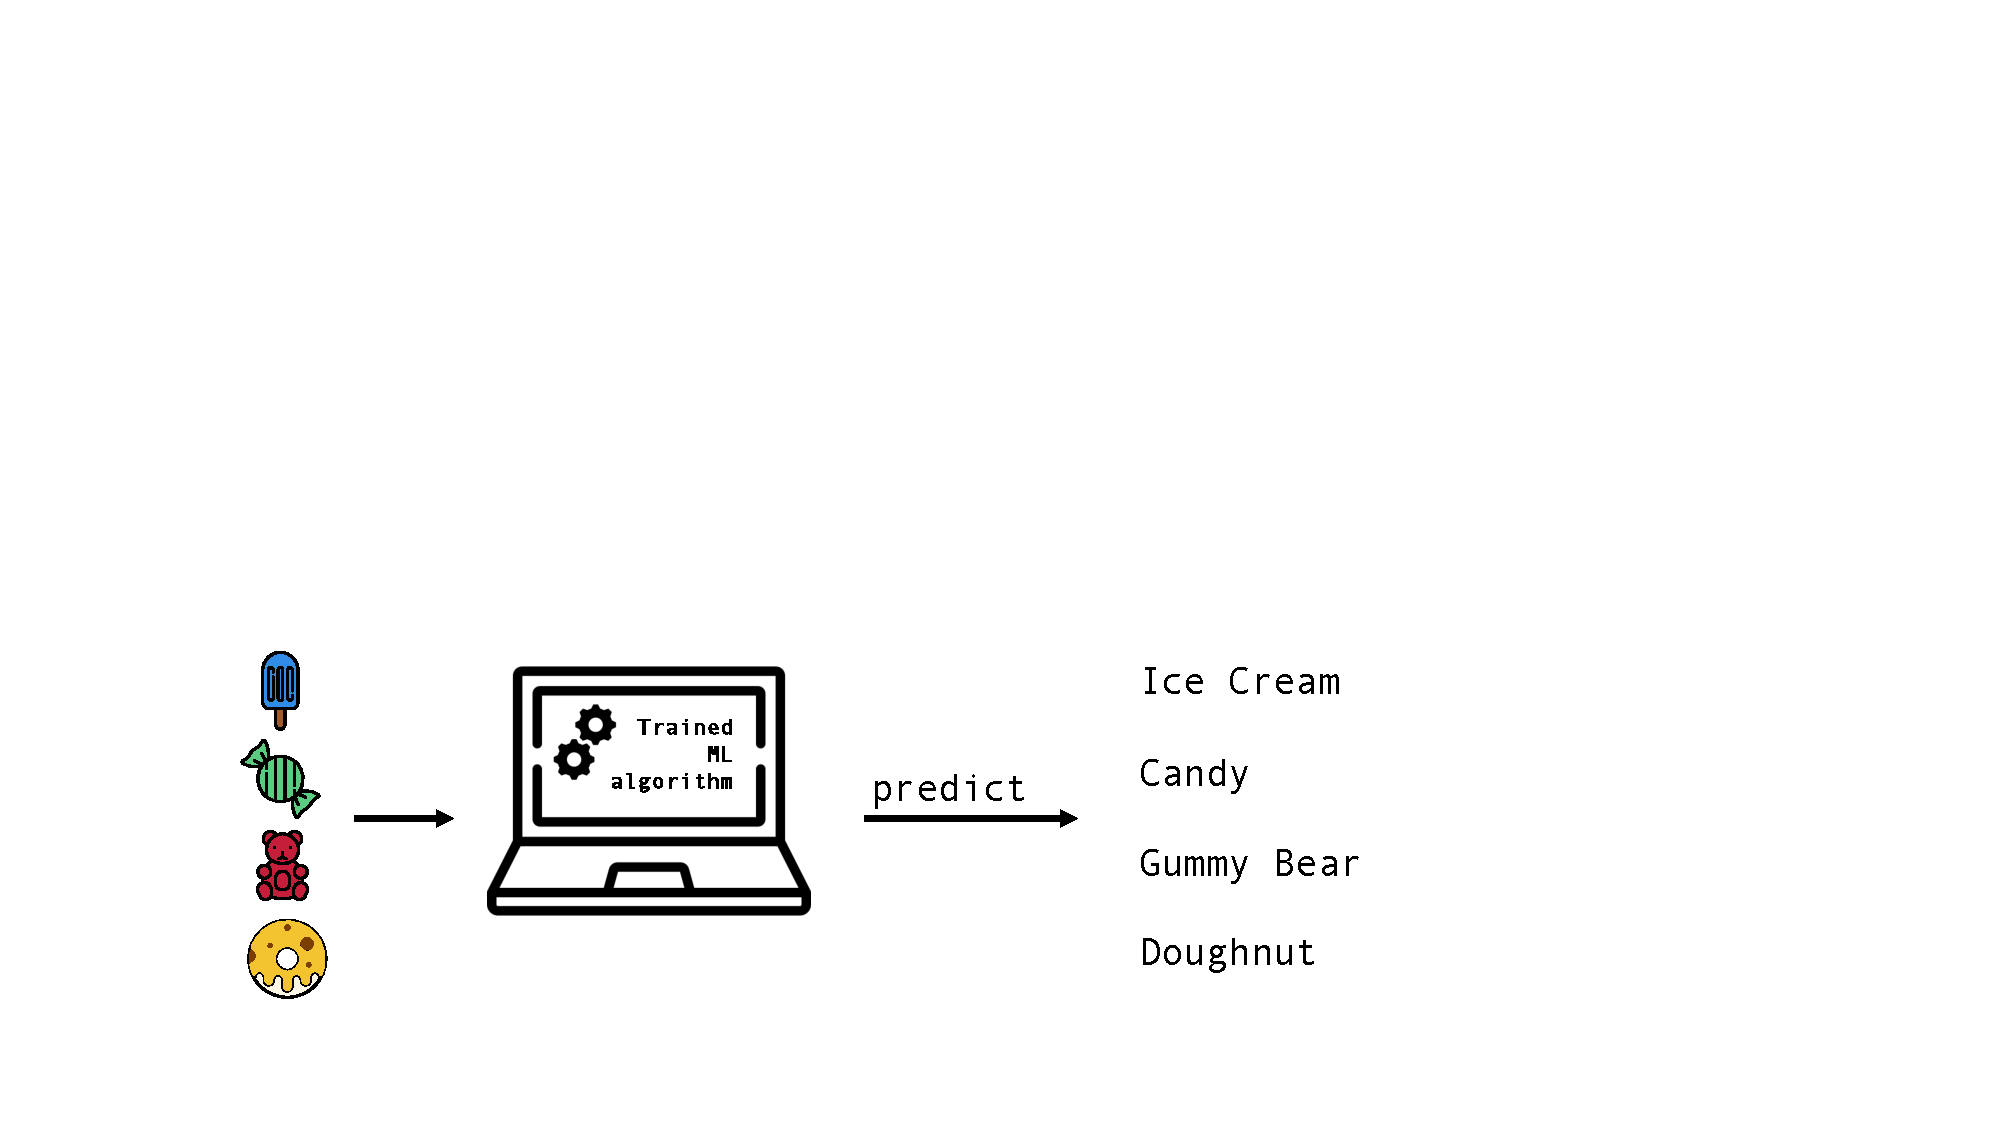
\includegraphics[scale=0.5]{Figures/example_prediction.pdf}
    \end{figure}
\end{frame}


\begin{frame}{Classification - Data Representation}
    \scriptsize
    \begin{columns}
        \begin{column}{0.8\textwidth}
            \centering
            \begin{tabularx}{0.8\textwidth}{@{}c|Y|Y|Y|Y@{}}
                \toprule
                    & \textbf{color} & \textbf{size [cm]} & \textbf{weight [g]} & \textbf{chocolate}  \\
                \midrule
                \parbox[c]{1em}{
\includegraphics[width=0.0175\textwidth]{Figures/023-gummy-bear-0.pdf}} & red & 2.02 & 1.99 & 0   \\
                \midrule
                 \parbox[c]{1em}{
\includegraphics[width=0.0175\textwidth]{Figures/023-gummy-bear-1.pdf}} & green & 1.98  & 2.10 & 0   \\
                \midrule
                \parbox[c]{1em}{
\includegraphics[width=0.0175\textwidth]{Figures/028-ice-cream-2.pdf}} & yellow & 14.20  & 56.15 & 1  \\
                \midrule
                \parbox[c]{1em}{
\includegraphics[width=0.0175\textwidth]{Figures/041-candy-3.pdf}} & blue & 2.45  & 4.30 & 0   \\
                \midrule
                \parbox[c]{1em}{
\includegraphics[width=0.0175\textwidth]{Figures/041-candy-1.pdf}} & green & 2.49  & 4.17 & 0  \\
                \midrule
                \multicolumn{5}{c}{$\vdots$}  \\
                \midrule
                \parbox[c]{1em}{
\includegraphics[width=0.0175\textwidth]{Figures/028-ice-cream-3.pdf}} & blue & 14.20  & 56.15 & 1 \\
                \midrule
                \parbox[c]{1em}{
\includegraphics[width=0.0175\textwidth]{Figures/046-donuts-2.pdf}} & yellow & 16.80  & 110.30 & 1  \\
                \bottomrule
            \end{tabularx}
        \end{column}
        \begin{column}{0.3\textwidth}
            \begin{tabular}{c}
                \toprule
                \textbf{label}  \\
                \midrule
                Gummy Bear   \\
                \midrule
                 Gummy Bear   \\
                \midrule
                Ice Cream   \\
                \midrule
                Candy   \\
                \midrule
                Candy   \\
                \midrule
                $\vdots$  \\
                \midrule
                Ice Cream   \\
                \midrule
                 Doughnut   \\
                \bottomrule
            \end{tabular}
        \end{column}
    \end{columns}

\end{frame}

\begin{frame}{Classification: Nearest Neighbor Classifiers}
    \begin{figure}
        \centering
        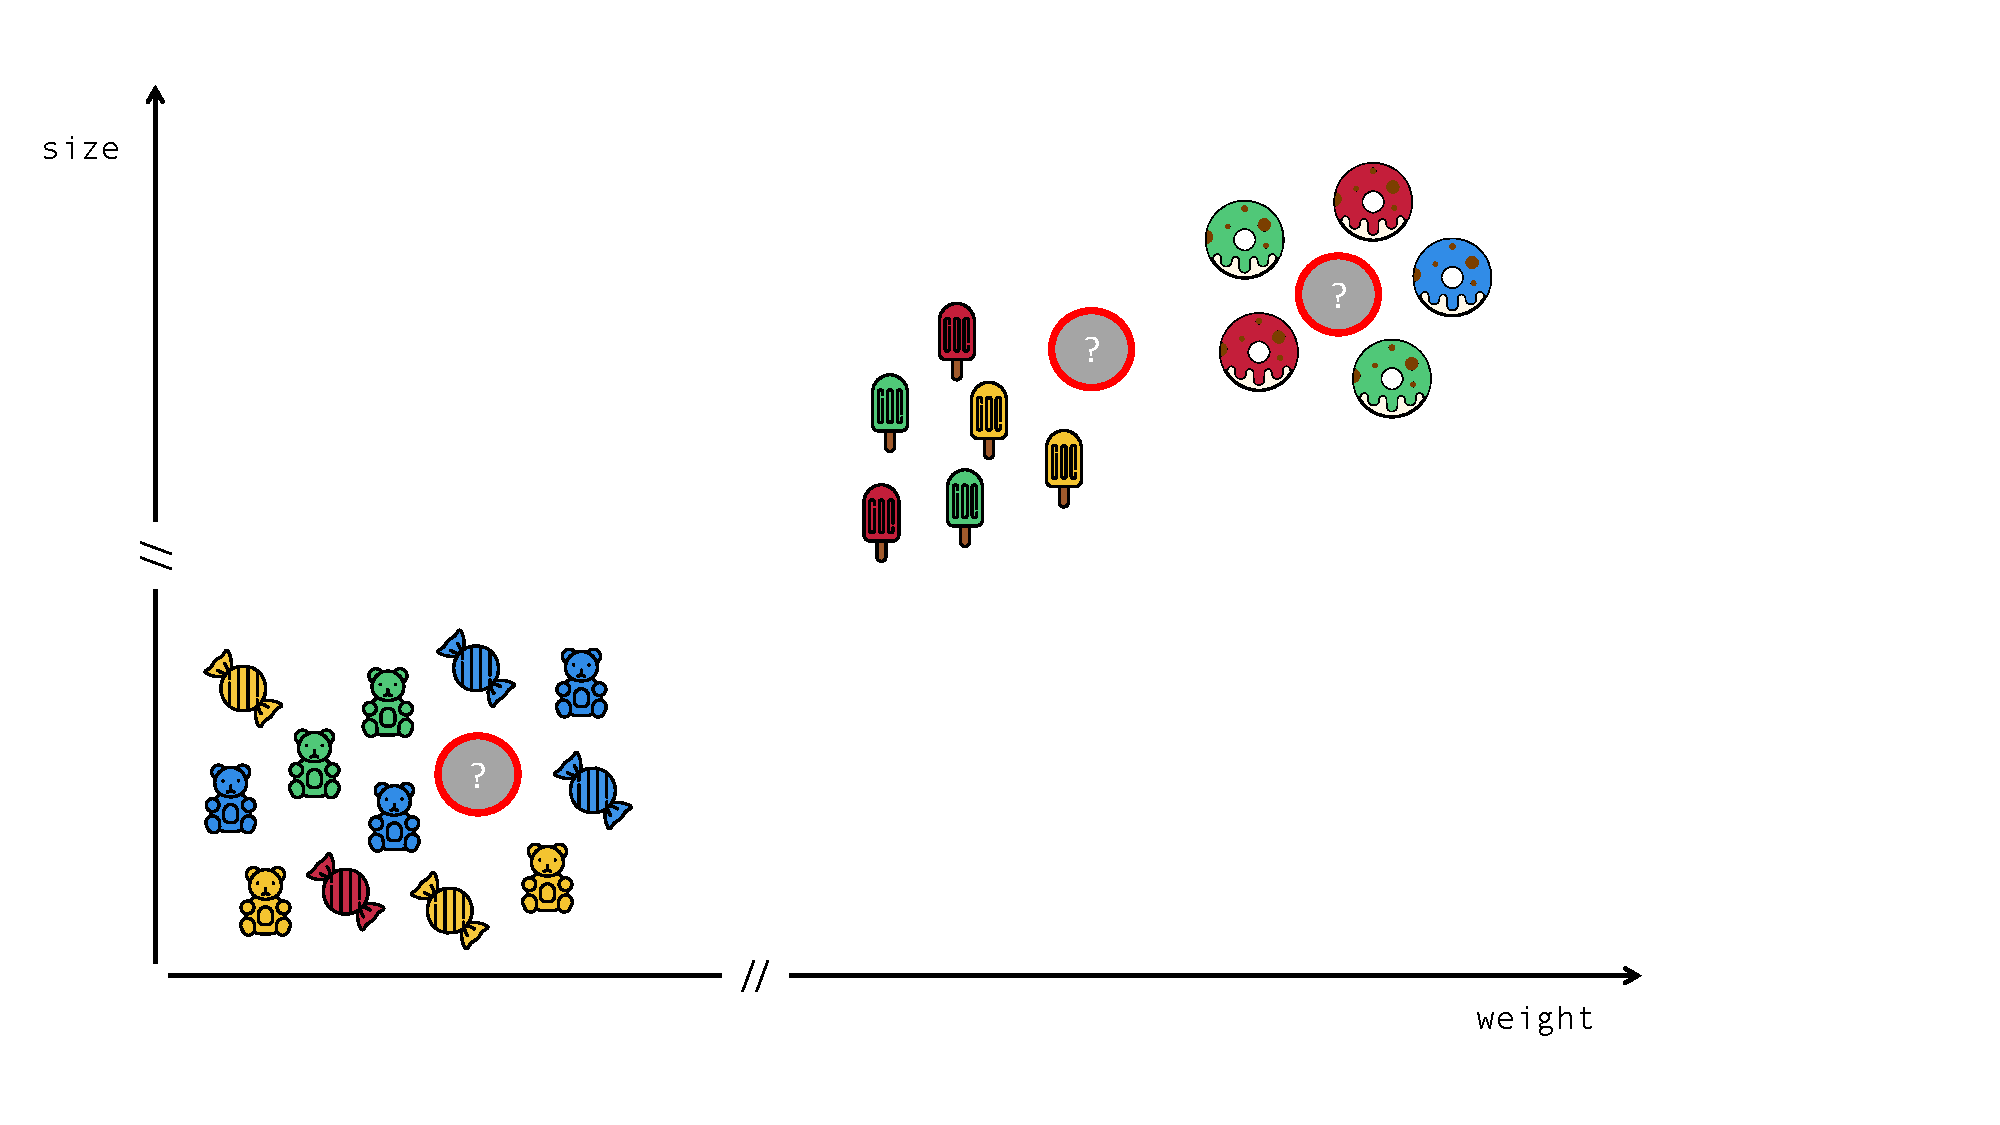
\includegraphics[width=0.8\textwidth]{Figures/example_kNN.pdf}
    \end{figure}
\end{frame}

\begin{frame}{Classification: Decision Tree Example}
    \begin{figure}
        \centering
        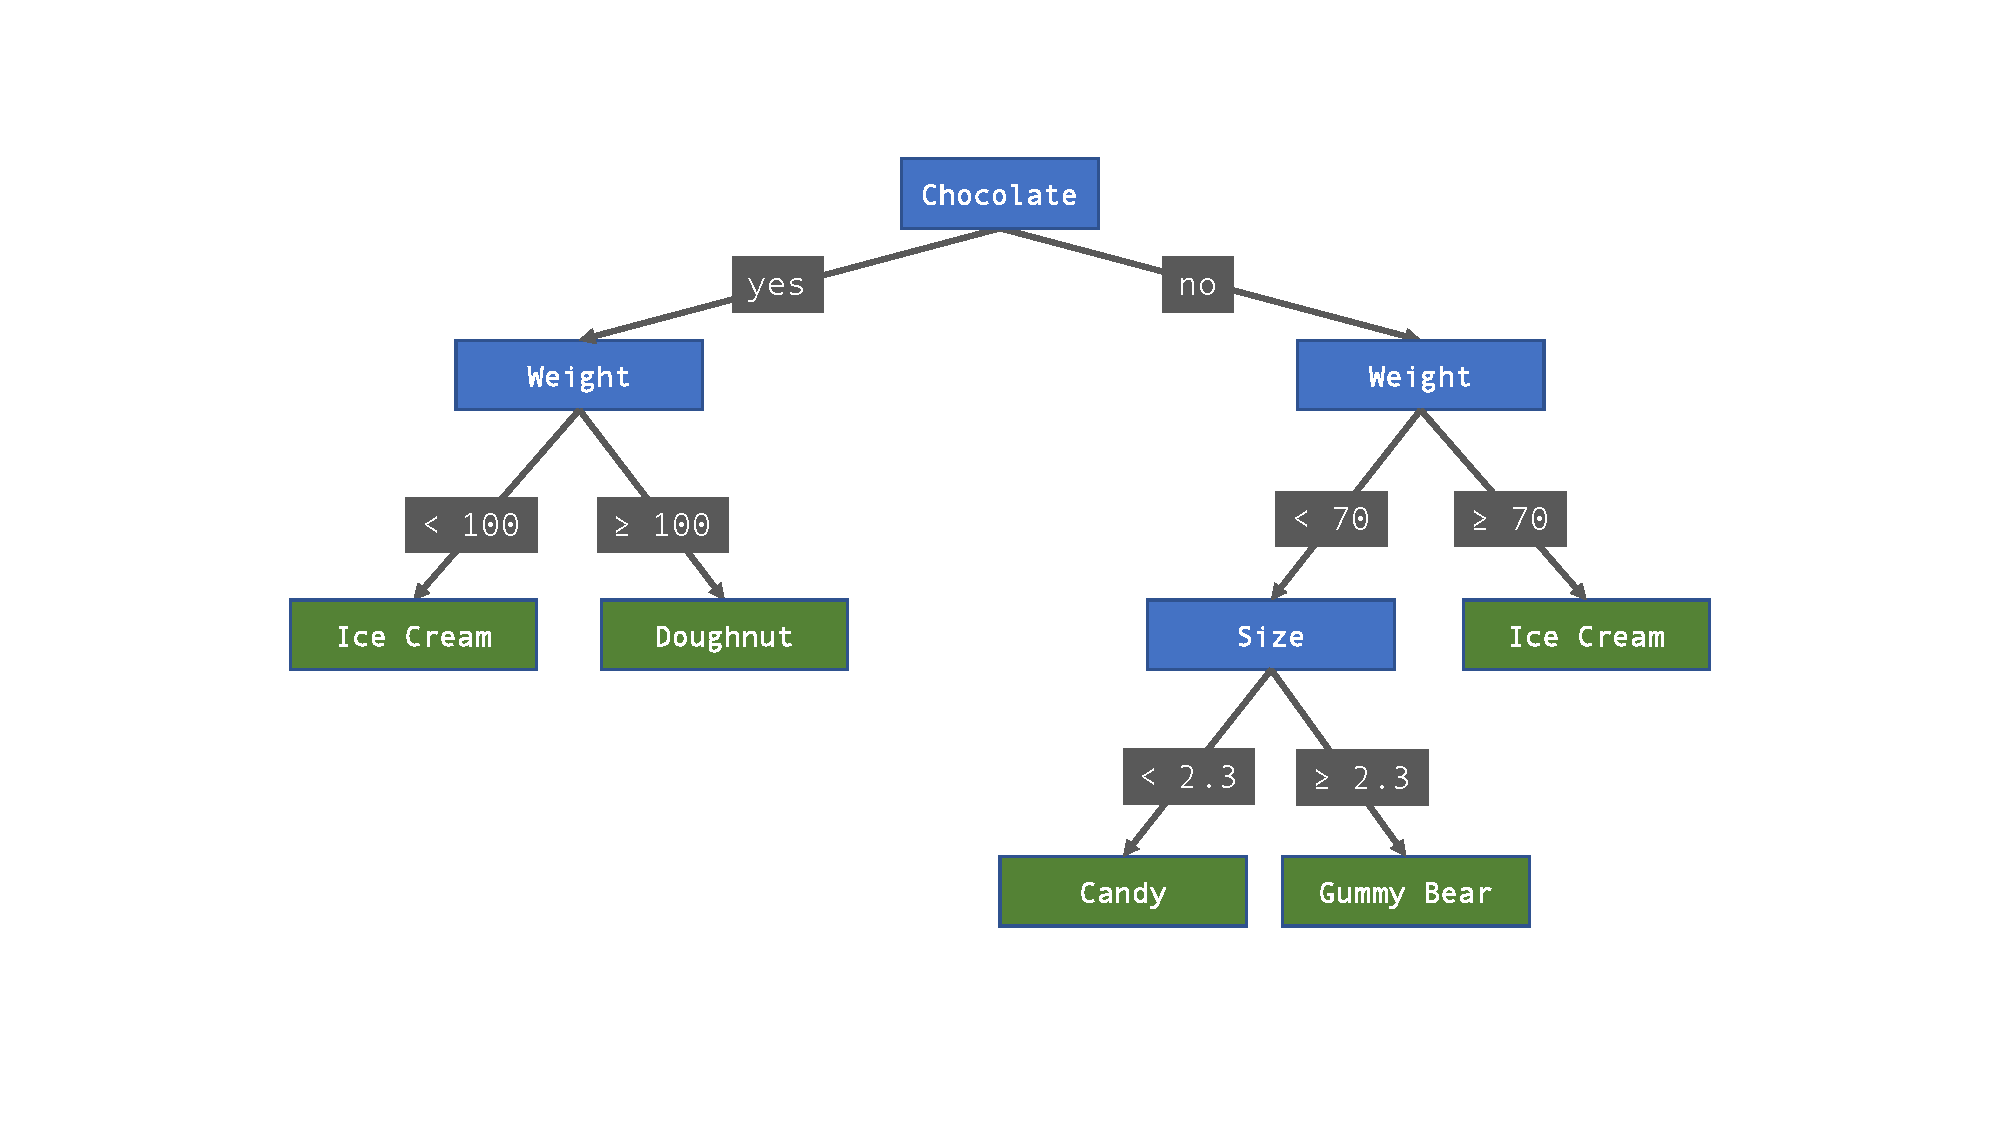
\includegraphics[width=0.8\textwidth]{Figures/example_decision_tree.pdf}
    \end{figure}
\end{frame}

\begin{frame}{Famous Classification Methods}
    \begin{itemize}
        \item Logistic Regression
        \item k-nearest Neighbor Classification (\textit{k}-NN)
        \item Naïve Bayes
        \item Support Vector Machines (SVM)
        \item Decision Trees and Random Forests
        \item Neural Networks
    \end{itemize}
\end{frame}

\begin{frame}{Classification vs. Regression}
    \begin{itemize}
        \item Very similar concepts and methods
        \item Instead of predicting a discrete \textit{class label} for
          each sample, predict a measurable \textit{continuous quantity}
    \end{itemize}
    \vspace{0.5cm}
    \textbf{Candy Regression}\newline
    The target to predict could become e.g.
    \begin{itemize}
        \item sugar content of a sweet
        \item calories
        \item ...
    \end{itemize}
\end{frame}

  \section{Common myths in machine learning}

  \begin{frame}{Myths in machine learning}
    \begin{enumerate}
      \item Machine learning does not need a clear objective.
      \item Machine learning does not need a clear hypothesis.
      \item Machine learning can extract the \emph{right} signal from your data.
    \end{enumerate}
  \end{frame}

  \begin{frame}{Machine learning needs clear objectives}
    \begin{block}{}
      Prior to applying any machine learning algorithm, you should have
      a clear objective in mind. Do you want to cluster data to learn
      about~(unknown) structures? Do you need to classify \emph{unseen}
      data in order to save valuable working time?
    \end{block}
    %
    \vfill
    %
    \textbf{Question}: What would an ``ideal'' algorithm do for \emph{your} project?
  \end{frame}

  \begin{frame}{Machine learning needs a hypothesis}
    \begin{block}{}
      Decide beforehand what you are looking for in your data. Do you
      hypothesise that a certain biomarker might exist in your data that
      is correlated with a phenotype? Do you hypothesise that there are
      subgroups of subjects of your study that give rise to similar
      behaviour?
    \end{block}
    %
    \vfill
    %
    \textbf{Take-away}: The results of a machine learning algorithm
    should be able to surprise you~(because a hypothesis has been
    disproved).
  \end{frame}

  \begin{frame}{Machine learning cannot extract something from nothing}
    \begin{block}{}
      If your data are very ``noisy'', the real signal might be
      hidden---and in the worst case, an algorithm might be unable to
      find it. Larger data sets might lead to better performance, but
      only if the data are properly curated.
    \end{block}
    %
    \vfill
    %
    \textbf{Take-away}: Be aware of inconsistencies in your data.
  \end{frame}


  \section{Your own projects}

\begin{frame}{Group Work 3: Discussion of individual projects (45min)}
    
    \textbf{Instructions:}
    \small
    \begin{itemize}
        \item What does your data look like (time series, images, genetic data, ...)?
        \item How large is the data set (number of samples/features)?
        \item Are there any pitfalls (high noise, missing data, incorrect measurements, ...)?
        \item What would you like to learn? What is the question you want to answer?
        \item Are you dealing with a clustering/classification/regression problem? What is your target variable?
        \item Can your question be answered with your current data set? If not, how would the data set have to be changed to answer the question (larger data set?        different experiments, ...)?
    \end{itemize}
\end{frame}

\begin{frame}{Question-Answer-Session}
    \begin{figure}
        \centering
        
\includegraphics[scale=0.3]{Figures/question_answer.eps}
    \end{figure}
\end{frame}

\begin{frame}{Machine Learning Resources}
    \scriptsize
    Online Resources:
    \begin{itemize}
        \item python's \texttt{scikit-learn} package plus documentation (hands-on ML techniques with examples)
        \item ML-lecture by A. Ng: https://www.coursera.org/learn/machine-learning
        \item \url{https://shapeofdata.wordpress.com}
    \end{itemize}
    \vspace{0.5cm}
    Textbooks:
    \begin{itemize}
        \item \textit{Elements of Statistical Learning} by T. Hastie, R. Tibshirani, J. Friedmann
        \item \textit{Machine Learning: a Probabilistic Perspective} by K. Murphy
        \item \textit{Understanding Machine Learning: From Theory to Algorithms} by S. Shalev-Shwartz, S. Ben-David
        \item \textit{Data Mining and Analysis: Fundamental Concepts and Algorithms} by  M.J. Zaki and W. Meira Jr.
        \item \textit{Data Mining: The Textbook} by C.C. Aggarwal
    \end{itemize}
    \vspace{0.5cm}
    \dots and of course: the Borgwardt-lab ;)
\end{frame}

  \begin{frame}{Acknowledgements}
    \begin{itemize}
      \item Icons were initially created by \href{https://www.freepik.com/home}{Freepik} from \href{https://www.flaticon.com}{www.flaticon.com}
      \item The machine learning breakdown figure was originally created
        by \href{https://robchavez.org}{Rob Chavez} and has been
        modified to fit into this course
    \end{itemize}
  \end{frame}

\end{document}
